\documentclass{article}
\title{Git Made Simple}
\author{Dmitri Priimak}
\date{}
\usepackage[a4paper,left=2.5cm, right=2.2cm, top=1.8cm, bottom=1.9cm]{geometry}
\usepackage{graphicx}
\usepackage{amsmath}  % extended mathematics
\usepackage{booktabs} % book-quality tables
\usepackage{units}    % non-stacked fractions and better unit spacing
\usepackage{multicol} % multiple column layout facilities
\usepackage{lipsum}   % filler text
\usepackage{fancyvrb} % extended verbatim environments
\usepackage{paralist}
\usepackage{amsthm}
\usepackage{fancyvrb}
\usepackage{tikz}
\usepackage{calc}
\usepackage{epstopdf}
\def\checkmark{\tikz\fill[scale=0.3](0,.35) -- (.25,0) -- (1,.7) -- (.25,.15) -- cycle;}
\def\scalecheck{\resizebox{\widthof{\checkmark}*\ratio{\widthof{x}}{\widthof{\normalsize x}}}{!}{\checkmark}}
\theoremstyle{definition}
\setcounter{secnumdepth}{2}
\begin{document}
       \newcommand{\segment}[1]{$\overline{#1}$}
       \newcommand{\msegment}[1]{\overline{#1}}
       \thispagestyle{empty}
       \begin{center}
           .

       \vspace{4cm}
       {\Huge \textbf{Hitchhikers Guide to Git}}

               \vspace{6mm}
       {\large by Dmitri Priimak

       v0.2
       }


       Creative Commons Attribution 4.0 International License


               \vspace{2cm}

       
\includegraphics[scale=0.4]{../../../target/images/giticon.pdf}
       \end{center}
       \newpage
       .
       \newpage
       \tableofcontents
       \newpage
       \setcounter{page}{1}
       \section{Introduction}
        Git is a source control tool primarily used for maintaining history, i.e. revisions of the source code. Unlike CVS or
        Subversion it can and does work without the server\footnote{It is common however to dedicate at least one instance
        of the Git repository as authoritative and expose it as a server.}. In those older source control tools server
        maintains complete history of the project, while clients (i.e. developers) have locally only one particular snapshot
        of that history. Git completely decentralizes history maintenance and therefore belongs to the category of
        distributed version control systems (aka. DVCS). To do that all DVCS maintain all history right next to the source
        code that they control, i.e. locally. There are many DVCS systems out there, such as Darcs\footnote{Notably Darcs
        does now allow merging where new commit has two parents but alway does rebase operation. You will read about merge
        and rebase operations later in the text.}, Mercurial, Bazaar and others, but only few survived the test time. The
        only other DVCS that still has any relevance is Mercurial. As far as having ability to maintain history of the
        source code Git is identical to Mercurial. Both use DAGs\footnote{Directed Acyclic Graphs} to represent history, but
        differ in how you interact with that history and in its underline representation. Critically they also differ in how
        you record new state in history. You also need to interact with the history if you wish to look or revert to earlier
        versions of the code, but you may also want to alter history for the purpose of presenting it without otherwise
        irrelevant details. In the approach that Git takes to history manipulation it differs greatly in philosophy from
        Mercurial, which takes dogmatic position that history is unalterable. Mercurial also allows you to do anything you
        may want with the history, but it tries very hard to make sure that you do not do that. In other words Mercurial gets
        in your way. Git freely exposes its "advanced" features while Mercurial tries to hide them from you. The side effect
        of that is that while gaining greater freedom with git you may also end up in a state of your repository that might
        appear confusing. Understanding git internals, or {\em plumbing}, allows you to be free of confusion in a situations
        like this and free to use git to your and everyone else benefit.

        Most of the git books start by talking about very high level commands (known in git-lingo as {\em porcelain})
        without explaining what actually happens under the hood. This often leads to familiarity with few commands that you
        will use every single day, but leaves large gray area of more advanced features because to understand them well you
        need to know the inner workings of git. A few manuals try to talk about inner working of git first, but usually nobody
        reads those kinds of texts. Here we will try to take a middle approach. We will talk about high level commands and
        then immediately refer to what actually happens under the hood, i.e. to the plumbing. There is also another impediment
        to understanding git. And that is a specific approach that some software developers, especially junior ones, take to
        the revision control tools, which is that developers often interact with git not by choice but due to necessity.
        Often in their minds eye they would like to see workings of revision control system to be completely invisible,
        something that happens in the background. Such system do exists, just think of your editor that has unlimited undo
        and replay actions, but they are very limited by that very simplicity of unguided interaction that users sometimes
        desire. Git takes completely different approach to recording revisions of the code you are working on. It requires
        all interactions with the history to be explicit, be that recording new revision or modifying history itself.
        This comes at the expense of some apparent complexity but in return you gain a lot of power. In reality git is a
        very simple and intuitive tool and you will think that way too once you understand how it works.

        Book "Pro Git"\footnote{You can read "Pro Git" book online here https://progit.org/ and here
        https://git-scm.com/book/en/v2 or get a dead tree version at your local bookstore.} and manual pages are the final
        authority on the workings of git. This booklet does not try to replace them in any way, but only to provide
        clarifications where author himself felt that, at least for him, better explanations are possible. Additionally
        writing of this booklet was driven by the idea that the best way to understand something is to try to explain it to
        someone else.

        Following major Git command will be described here:

        \begin{center}
        \begin{tabular}{ l l l }
        $\bullet$ init & $\bullet$ branch & $\bullet$ checkout \\
        $\bullet$ commit & $\bullet$ clone & $\bullet$ reset \\
        $\bullet$ push & $\bullet$ pull & $\bullet$ merge \\
        $\bullet$ status & $\bullet$ diff & $\bullet$ log \\
        $\bullet$ fetch & $\bullet$ rebase
        \end{tabular}
        \end{center}

        \newpage
        \section{Work tree and its state}
        At the highest level of abstraction git allows you to take a directory with some files in it and turn into
        something akin to versioning file system. Then you can record state of your directory, also known as work tree.
        You can then restore your work tree to any state that you have recorded in the past and even modify its
        history. And as I already mentioned before, git does not get in your way if modifying history is what you are
        after. What you track is actually files in the tree not directories and you have to explicitly specify that you
        want to track state of any particular file. If you do not request git to track state of some file than git does
        not know anything about it and if you delete it git will not help in restoring it. For the files for which git
        tracks state situation is different. If you delete such file git will allow you to restore to any of its
        recorded states. Thus when git looks at the file it classifies it into one of three major categories
        \begin{enumerate}
                \item Untracked - git knows nothing about this file.
                \item Unmodified - git tracks state of this file and it is the same as the slice of history you are looking it.
                \item Modified - git tacks this file and it is now different from what is recorded in git.
        \end{enumerate}
        If you read other books you probably saw that there is another state for tracked files, which is {\em Staged}.
        I do not list it here because it is in a way a form of {\em Modified} state. You will learn about it later when
        we will understand how git records new state of the work tree.

        \section{A bit of plumbing}
        Git repository is contained in \texttt{.git/} directory at the top of the source code under control of the git. When
        discussing higher abstraction git commands we will be immediately referring to files under \texttt{.git/} rather
        than saying nothing about them.

        At a certain level of abstraction git is nothing else but a sequence of commits. Commit represents a state of the
        source code at the time it was created and it consist of following three parts:
        \begin{enumerate}
            \item Commit object that describes the patch set, i.e. when it happened, who did it, pointer to the parent commit and pointer to the tree object.
            \item A tree object that contains pointers to the files associated with this commit.
            \item Set of files, each stored as a zlib compressed blob.
        \end{enumerate}
        All objects described above are stored in the files whose names are SHA1 hash values and when we say pointer to some
        file or object that pointer is SHA1 hash value of corresponding object. These SHA1 hash values are computed based
        on content of the blobs. Therefore a commit object is also just a file with name that is its SHA1 hash. This allows one
        to form tree of objects like so.

        \begin{figure}[h]
        \centering
        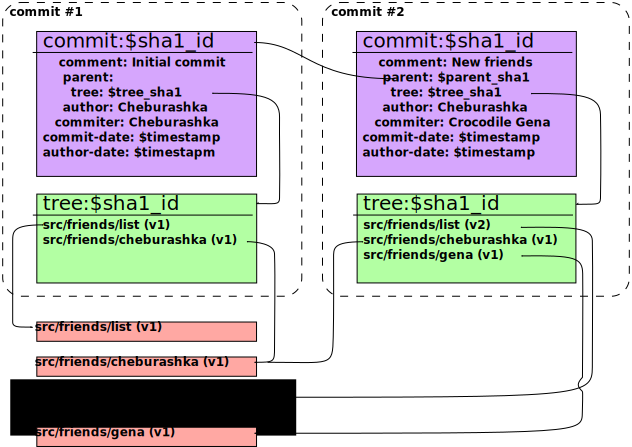
\includegraphics[scale=0.59]{../../../target/images/patch-set.pdf}
        \label{fig:patch-set}
        \caption{Three types of objects (files) forming commit. They are {\em commit}, {\em tree} and {\em blob}. The later
          one holds content of the files tracked by git, i.e. under control of git.}
        \end{figure}

        \noindent Notice that different commits do share pointers the same files where possible. References to files are
        also SHA1 values since content is stored in files with names that are these SHA1 values. That is all there is to how
        git stores state of the work tree. Git repository can contain many trees like this. They are known as branches. When
        trees do not share common ancestor they are known as "{\em disconnected branches}". Actually in Git branches have
        more restricted meaning then that and in the next chapter we will see what that meaning is.

        \section{Branches}

        Obviously navigating these branches by SHA1 values is not very user friendly. To help with that git provides a set
        of symbolic names that point to specific commits within existing branches. Users can also create symbolic names or
        references that point to arbitrary commits or other symbolic names. We will speak of these names as {\em refs}
        unless using formal {\em symbolic reference}. Whenever you initialize new Git repository you automatically create
        one ref that points to the head of the tree to be formed. That reference identifies the branch and allows you to refer
        to that branch by its reference, i.e. a name. Actually in git that reference is the branch. This is fundamentally
        different from Mercurial, which maintains special branch label with each commit. This means that in Mercurial you
        can always know to which branch commit actually belongs. In git that is often not possible. Once loops in history
        are created by means of merge and now useless references are removed there is no way to know on which branch a
        certain commit is. These linear strands of history in git are of course real branches in the same sense as in
        Mercurial, but in git they do not have any special permanently frozen identifiers. So called branch references in
        git are just pointers into sequence of commit from which history can be extended by adding new commits. It is
        however common in the git world to speak of branch reference as the branch itself and in the simplest cases they do
        match with real branches as you find them in Mercurial but really these are two different things.

        When repository is freshly initialized default branch (aka. branch reference) is created and it has name
        \texttt{master}. Also cerated is ref \texttt{HEAD} which refers to the \texttt{master} as you can see in the
        example on the following figure.

        \begin{figure}[h]
            \centering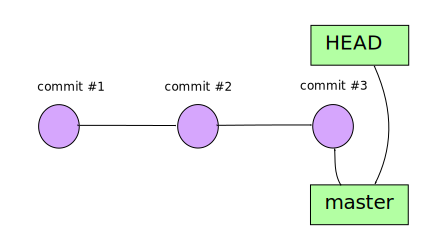
\includegraphics[scale=0.6]{../../../target/images/one-branch.pdf}
            \caption{Simple linear branch consisting of three commits. Symbolic reference \texttt{master} points to the last
              commit of the branch. Symbolic reference \texttt{HEAD} points to sym. reference \texttt{master}.\label{fig:one-branch}}
        \end{figure}

        \noindent The commit to which \texttt{HEAD} refers to directly or indirectly is what is considered to be currently
        {\em checked out commit}. It will commonly be the case that files in your work tree do match with checked out
        commit, i.e. they in Unmodified state, but they can also be in Modified state if well ... you modify them.

        So, lets play around with git and see how it works. Imagine that we decided to start a project which will
        accumulate computer related pearls of wisdom. We will call it \texttt{wisecracks}. We create directory with that
        project name and initialize new repository for it and see what it looks like. We do that by using git command
        {\em init}\footnote{Git provides extensive help for each command, which you can see in the terminal by
        appending \texttt{--help} to any command. For example \texttt{git init --help}}.

        \begin{Verbatim}[frame=single]
 $ mkdir ~/wisecracks && cd ~/wisecracks/
 $ git init .
        \end{Verbatim}
        This creates directory \texttt{.git/} which is where history of the files you work with will be held. If you now
        look there you will find bunch of files and directories. Specifically if you look into file \texttt{HEAD} will
        see following

        \begin{Verbatim}[frame=single]
 $ cat .git/HEAD
 ref: refs/heads/master
        \end{Verbatim}
        This is your current branch. String \texttt{refs/heads/master} refers to an actual file. But you do not really have
        any commits in your repository and therefore this file does not exist. File \texttt{refs/head/master} would contain
        SHA1 of the last commit and since we do not have any that ref does not exist either.

        Before we will proceed with our first commit we will set some git parameters which will be used when making a
        commit. As a matter of fact git will refuse to do commit unless commiter email and name are set. Following
        commands will set these parameters for this repository only\footnote{You will find these and other parameters in
        the file \texttt{.git/config}}

        \begin{Verbatim}[frame=single]
 $ git config user.email 'smarty.pants@shmoogle.com'
 $ git config user.name 'Mr. Smarty Pants'
        \end{Verbatim}
        Now, lets add file \texttt{Quotes}, create first commit and see what happens.

        \begin{Verbatim}[frame=single]
 $ echo "Beware of computer programmers that carry screwdrivers." > Quotes
 $ git add Quotes
 $ git commit -m 'Initial commit.'
 [master (root-commit) f589b63] Initial commit.
  1 file changed, 1 insertion(+)
    create mode 100644 README
        \end{Verbatim}

        Do not worry about "\texttt{git add}" line, we will get to that later. For now you just need to know that this
        creates commit which looks very much like what you see in Figure 2 above, except that there is only one commit. If
        we look at the file \texttt{refs/heads/master} we will see following\footnote{Even if you follow instructions
        provided here exactly, due to the way git generates sha1 values ref shown in the example here will be different.
        Thus you need to adjust for that when repeating these steps. SHA1 values for commits will be different from what
        you will encounter in this book because commit includes two timestamps for when the patch/commit was created and
        when it was applied, but SHA1 values for other objects such as trees and blobs (files) will be exactly as show
        in the text.}

        \begin{Verbatim}[frame=single]
 $ cat .git/refs/heads/master
 f589b633fe518cd5fba61d03a7e0087015f0b27e
        \end{Verbatim}

        Now ref \texttt{master} does point to some commit. There is actually a file with name derived from this long
        string and it is located at \texttt{.git/objects/f5/89b633fe518cd5fba61d03a7e0087015f0b27e}. The file is zlib
        compressed and while you can actually uncompress it manually to see what is inside git provides convenient
        command {\em cat-file}. We can use it to find type of the object/file referred to by a particular SHA1 value.

        \begin{Verbatim}[frame=single]
 $ git cat-file -t $(cat .git/refs/heads/master)
 commit
        \end{Verbatim}
        And see what is inside of the that object

        \begin{Verbatim}[frame=single]
 $ git cat-file -p $(cat .git/refs/heads/master)
 tree 87dee0e56fef3545d952a43d29e0f64ccca80424
 author Mr. Smarty Pants <smarty.pants@shmoogle.com> 1463030863 -0700
 committer Mr. Smarty Pants <smarty.pants@shmoogle.com> 1463030863 -0700

 Initial commit.
        \end{Verbatim}
        Notice that content of the {\em commit} object has SHA1 reference to a {\em tree} object. We can now follow these
        references\footnote{You do not actually have to use whole SHA1 value to identify and retrieve an object. You can use
        minimum necessary number of character to uniquely identify object. That can be just a couple of first characters
        of SHA1 value. Notice that after many operations git prints out just first 7 characters, which in a wast majority of
        the cases is sufficient.} to identify all parts of the commit, which you can see in Figure 1.

        \begin{Verbatim}[frame=single]
 $ git cat-file -t 87dee0e56fef3545d952a43d29e0f64ccca80424
 tree
 $ git cat-file -p 87dee0e56fef3545d952a43d29e0f64ccca80424
 100644 blob f97afbc4595b699467b4bee351d7f66a23336671   Quotes
        \end{Verbatim}
        You can see that type of tree object is, well a {\em tree} and it contains a reference to a single object
        within that tree, which is our file \texttt{Quotes}. And if we follow into that object we will see

        \begin{Verbatim}[frame=single]
 $ git cat-file -t f97afbc4595b699467b4bee351d7f66a23336671
 blob
 $ git cat-file -p f97afbc4595b699467b4bee351d7f66a23336671
 Beware of computer programmers that carry screwdrivers.
        \end{Verbatim}
        We realize now that we forgot to attribute this quote and decide to fix that.

        \begin{Verbatim}[frame=single]
 $ echo "    - Leonard Brandwein" >> Quotes
 $ git add Quotes
 $ git commit -m 'Added attribution.'
 [master fdf4045] Added attribution.
  1 file changed, 1 insertion(+)
        \end{Verbatim}
        Now a branch reference points to another commit and that commit now has a parent.
        \begin{Verbatim}[frame=single]
 $ git cat-file -p $(cat .git/refs/heads/master)
 tree 42164ddfe47567d0fbf508167de3b436088f5861
 parent cf82886ebef5ffc891f2014466c26f7b9760db59
 author Mr. Smarty Pants <smarty.pants@shmoogle.com> 1463032203 -0700
 committer Mr. Smarty Pants <smarty.pants@shmoogle.com> 1463032203 -0700

 Added attribution.
        \end{Verbatim}

        \noindent Thus we have a chain, or a branch, consisting of two commits. One more commit and our history will
        look exactly like in Figure \ref{fig:one-branch}.

        Now let us try to understand how commit is created. This will naturally explain what \texttt{git add} command
        does. Lets modify our \texttt{README} file some more and also add another file.

        \begin{Verbatim}[frame=single]
 $ echo "Never trust a computer you can’t throw out a window." >> Quotes
 $ echo '#!/usr/bin/ruby\nputs "Hallo"' > speak.rb
 $ chmod 755 speak.rb
        \end{Verbatim}
        We now have two files in our source code, a modified \texttt{Quotes} and new \texttt{speak.rb}. We can use
        "\texttt{git status}" command to see how our source differs from a particular slice of the recorded history.

        \begin{Verbatim}[frame=single]
 $ git status
 On branch master
 Changes not staged for commit:
   (use "git add <file>..." to update what will be committed)
   (use "git checkout -- <file>..." to discard changes in working directory)

         modified:   Quotes

 Untracked files:
   (use "git add <file>..." to include in what will be committed)

         speak.rb

 no changes added to commit (use "git add" and/or "git commit -a")
        \end{Verbatim}

        \noindent This says that file \texttt{Quotes} is indeed modified and that git knows nothing with regards to file
        \texttt{speak.rb}. However this output is quite verbose and it is common to use "\texttt{git status -s}" which
        shows the same information in very concise format

        \begin{Verbatim}[frame=single]
 $ git status -s
  M Quotes
 ?? speak.rb
        \end{Verbatim}
        This means exactly the same as what is shown above. Run "\texttt{git status --help}" to learn how to read this
        abbreviated output. However we will continue using default long format of "\texttt{git status}" in our examples.
        \newpage

        \noindent To see how your files differ from currently checked out commit you can use "\texttt{git diff}" command
    \begin{Verbatim}[frame=single]
 $ git diff Quotes
 diff --git a/Quotes b/Quotes
 index 773b2c9..247bf33 100644
 --- a/Quotes
 +++ b/Quotes
 @@ -1,2 +1,3 @@
  Beware of computer programmers that carry screwdrivers.
      - Leonard Brandwein
 +Never trust a computer you can’t throw out a window.
        \end{Verbatim}
        This will actually show difference between file in your work tree and something called {\em git index}. We will
        learn about index in the next chapter and will come back to see how "\texttt{git diff}" actually works, however in
        the state we find ourselves right now this is the same as difference between your modified files and how they
        were in the last commit. You can also launch external gui diff tool\footnote{This command will prompt with
          graphical diff tool that it will find in the filesystem, this can \texttt{meld}, \texttt{tkdiff} etc.} from
        the command like so:

        \begin{Verbatim}[frame=single]
 $ git difftool Quotes
        \end{Verbatim}
        But now you will encounter one major difference from Mercurial. If you try to commit your changes right now
        nothing will actually happen!

    \begin{Verbatim}[frame=single]
 $ git commit -m 'New quote and speak.rb'
 On branch master
 Changes not staged for commit:
        modified:   Quotes

 Untracked files:
        speak.rb

 no changes added to commit
        \end{Verbatim}
        Message that you got back tells you that while there are changes in your working tree nothing is actually
        committed and history is not recorded. With git you need to specify explicitly what it is you wish to record
        in the next commit. This is actually very convenient feature of git. In sufficiently large code tree you may
        work on several subcomponents and be done and ready to commit work done on one subcomponent and not another.
        With git unlike Mercural this is a trivial operation.

        \section{Git Index}

        In git you need to pre-bake your commit by recording state of your filesystem tree that you wish to commit first
        and then perform commit. Recording state that is needed to form new commit is done in file \texttt{.git/index},
        which often simply referred to as {\em git index} or {\em git staging area}. As a matter of fact git index
        always contains record of certain state of the filesystem tree, which is expressed through set of SHA1 values of 
        blobs referenced in the index. When you just made new commit or checked out
        certain commit, index contain the same references as that commit. As you work, state of you work tree will diverge
        from the state recorded in the index. In our example, in the current state file \texttt{Quotes} differs from file
        referenced in the index and file \texttt{speak.rb} cannot be found in any of the tree objects maintained by git.
        But git index might also diverge from the state recorded in currently checkout commit. We will see soon how it
        might happen. To help you visualize this you need to think of three main logical entities which are:
        \begin{enumerate}
                \item Your current source code tree, aka. work tree.
                \item Set of commits organized in branches that track history of our work tree
                \item Git index\footnote{Name "git index" is a strange one and many people will prefer to speak of index as a {\em staging area}.}
        \end{enumerate}
        \newpage
        \noindent After the last changes that you made in the work tree current state of your repository looks like so:
        \begin{figure}[h]
        \centering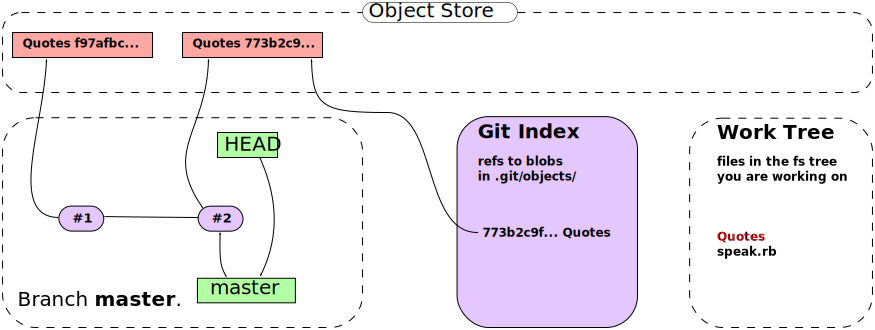
\includegraphics[scale=0.6]{../../../target/images/history-tree-index.pdf}
        \caption{Locally file \texttt{Quotes} is modified (this fact is indicated by the red font color) and file
          \texttt{speak.rb} added, but these changes are not recorded by git in any shape or form.\label{fig:history-tree-index}}
        \end{figure}

        \noindent You can see content of the index by using "\texttt{git ls-files}" command.

    \begin{Verbatim}[frame=single]
 $ git ls-files -s
 100644 773b2c9f72575404e5dfe92a3d596dca9da9ca2e 0      Quotes
        \end{Verbatim}

        \noindent In index SHA1 value for \texttt{Quotes} is exactly the same as recorded in the last commit. You can
        think of index as ephemeral commit. Most of the time it is the same as currently checked out one, but can
        become different from it when new state is recorded by means of "\texttt{git add}" operation. There are other
        operations such as "\texttt{git checkout}" that can make index diverge from currently checkout commit
        (i.e. \texttt{HEAD}), but we will talk about them later. To create commit we need to stage current state of work
        tree into the index by using "\texttt{git add}" command.

    \begin{Verbatim}[frame=single]
 $ git add Quotes speak.rb
 $ git status
 On branch master
 Changes to be committed:
   (use "git reset HEAD <file>..." to unstage)

        modified:   Quotes
        new file:   speak.rb
        \end{Verbatim}

        \begin{figure}[h]
        \centering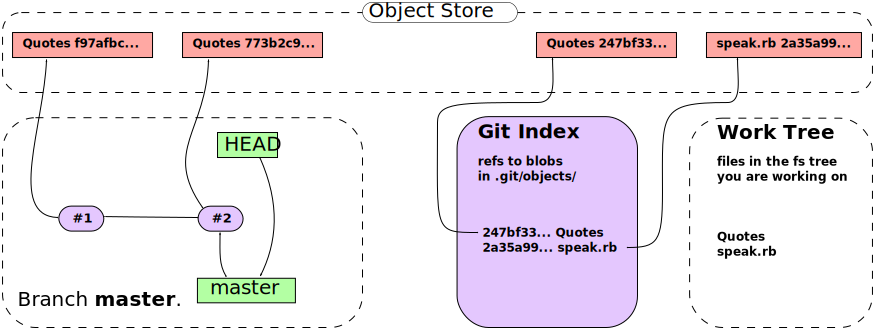
\includegraphics[scale=0.6]{../../../target/images/history-tree-index-staged-1.pdf}
        \caption{Files \texttt{README} and \texttt{hallo.rb} are recorded in index and in the object store, i.e.
          content of two blobs \texttt{247bf33} and \texttt{2a35a99} is the same as in the work tree. Index now
          diverged from the latest recorded state (i.e. commit) in the \texttt{master} branch.
          \label{fig:history-tree-index-staged-1}}
        \end{figure}

        \noindent Interestingly if you now run "\texttt{git diff Quotes}" you will see no output. The reason is that by
        default diff is computed against files recorded in the index and the work tree and currently what is
        recorded in the index exactly matches what is in the work tree. To see difference between last commit and what
        is in your work tree you can run:

    \begin{Verbatim}[frame=single]
 $ git diff HEAD Quotes
 diff --git a/Quotes b/Quotes
 index 773b2c9..247bf33 100644
 --- a/README
 +++ b/README
 @@ -1,2 +1,3 @@
  Beware of computer programmers that carry screwdrivers.
      - Leonard Brandwein
 +Never trust a computer you can’t throw out a window.
        \end{Verbatim}

        \noindent This output you already seen. But wait, we forgot to attribute last quote. Lets fix that.

    \begin{Verbatim}[frame=single]
 $ echo "    - Steve Wozniak" >> Quotes
 $ git status
On branch master
Changes to be committed:
  (use "git reset HEAD <file>..." to unstage)

        modified:   Quotes
        new file:   speak.rb

Changes not staged for commit:
  (use "git add <file>..." to update what will be committed)
  (use "git checkout -- <file>..." to discard changes in working directory)

        modified:   Quotes
        \end{Verbatim}
        This might look a bit strange. File \texttt{Quotes} appears as modified twice but it is actually very simple. The
        second appearance of \texttt{"modified: Quotes"} indicates that our work tree diverged from what is recorded in
        the index. If we will run "\texttt{git diff Quotes}" right now we will see difference between index and the work tree.

    \begin{Verbatim}[frame=single]
 $ git diff Quotes
diff --git a/Quotes b/Quotes
index 247bf33..a78fe2a 100644
--- a/Quotes
+++ b/Quotes
@@ -1,3 +1,4 @@
 Beware of computer programmers that carry screwdrivers.
     - Leonard Brandwein
 Never trust a computer you can’t throw out a window.
+    - Steve Wozniak
        \end{Verbatim}
        If we are to perform commit right now then only what is recorded in the index will go into the new commit. The
        last line "\texttt{- Steve Wozniak}" will NOT go into that commit! To review one more time what it is you would
        be committing you can run "\texttt{git diff --staged}"\footnote{You can also use option \texttt{--cached},
          which is a synonym for \texttt{--staged}}, which will show difference between HEAD and what is recorded in
        the index. It is most likely that you actually want to commit file \texttt{Quotes} with all the changes that
        you have made so far including attribution to Steve Wozniak. To do that you need to run
        "\texttt{git add Quotes}" one more time.

    \begin{Verbatim}[frame=single]
 $ git add Quites
 $ git status
On branch master
Changes to be committed:
  (use "git reset HEAD <file>..." to unstage)

        modified:   Quotes
        new file:   speak.rb
        \end{Verbatim}
        This will create new blob object that contains current state of file \texttt{Quotes} in the work tree and
        update index to contain reference to it. And now our repository looks like so:

        \begin{figure}[h]
            \centering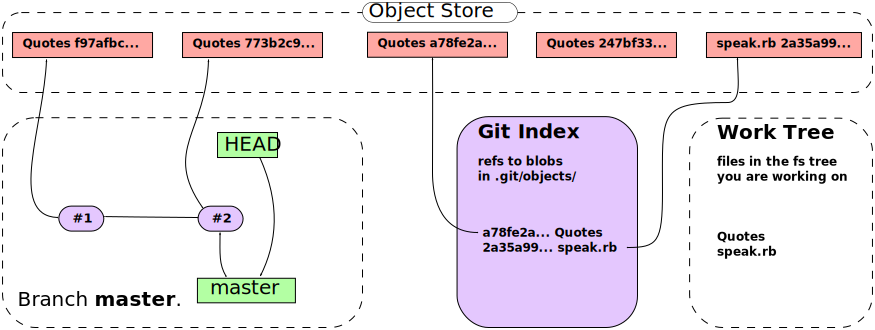
\includegraphics[scale=0.6]{../../../target/images/history-tree-index-staged-2.pdf}
            \caption{File \texttt{README} and \texttt{hallo.rb} are fully recorded in index and in the object store.\label{fig:history-tree-index-staged-2}}
        \end{figure}

        \noindent But there is something strange about this picture. There is orphan blob object that at some point
        recorded state of file \texttt{Quotes} but is no longer needed. You can still retrieve it by using
        "\texttt{git cat-file}" command. As matter of fact git will maintain many such dangling objects and even
        references to them in something called \texttt{reflog}, which means that you can actually undo many of
        operations that seemingly ruin you work tree and even recorded history. Git will eventually delete these orphan
        files, but you can clean them up right now by running \texttt{git gc} command. Obviously once orphaned objects
        and commit are removed any damage that you have done to the local repository is permanent. Now let us do garbage 
        collection and perform commit.

    \begin{Verbatim}[frame=single]
 $ git gc --prune=now
 $ git commit -m 'New quote and speak.rb'
 [master 3ab9407] New quote and speak.rb
  2 files changed, 4 insertions(+)
  create mode 100755 speak.rb
        \end{Verbatim}
        You can verify now that orphaned file is gone and the new state of the repository looks like this

        \begin{figure}[h]
        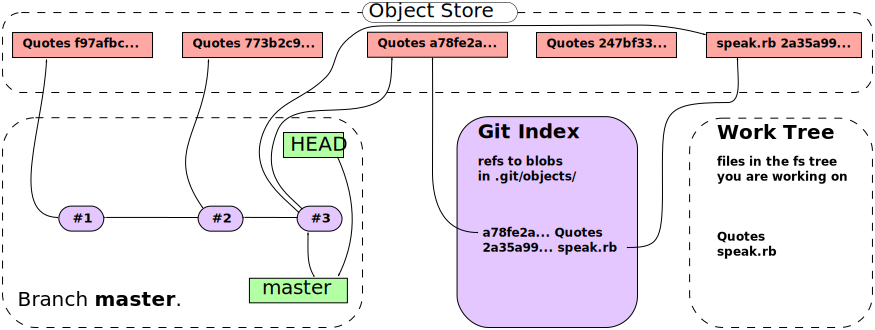
\includegraphics[scale=0.6]{../../../target/images/history-tree-index-committed.pdf}
        \caption{State our repository and work tree right after gc and third commit.\label{fig:history-tree-index-committed}}
        \end{figure}

        It important to note that whenever we do "\texttt{git checkout}" or make new commit the index is made to look
        exactly as currently checked out commit. It is only when we prepare new commit then for a brief period of time
        index diverges from previously checked out commit.

        \section{Git Checkout}

        We recorded history but now we would like to look at how our code looked like several commits back.
        Before we do that lets look at the current state of our repository and the work tree in more abbreviated form.

        \begin{figure}[h]
        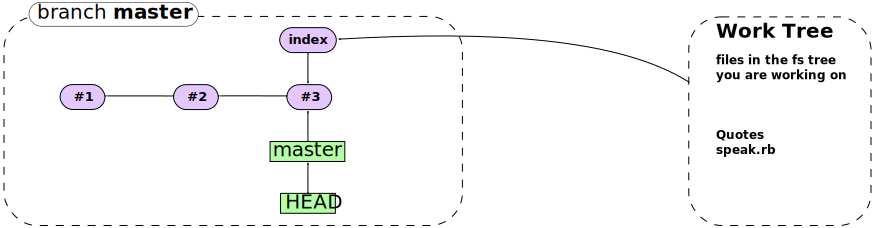
\includegraphics[scale=0.6]{../../../target/images/commits-3.pdf}
        \caption{Abbreviated form representing state our repository and work tree right after third commit.\label{fig:commits-3}}
        \end{figure}

        \noindent Remember, index is very much like ephemeral commit that most of the time identical to currently
        checked out commit. To express that we show it to be the same color as existing commits. When index
        diverges from that commit we will show it in red. State of the work tree is often compared against index, which is
        why link from the work tree goes to the  index. When work tree diverges from index we show that link as dashed
        line and modified files in bold.

        To travel back in time we will use "\texttt{git checkout}" command. It allows us to make our work tree look
        exactly as it was recorded in any particular commit. Let see what happens when we checkout the very first
        commit in our branch. We can do that in several ways. More rudimentary way is to find SHA1 of the fist
        commit. To that end we can use "\texttt{git log}" command.

        \begin{Verbatim}[frame=single]
 $  git log --graph --decorate --pretty=oneline
 * bfafe95af909d2c5a643fad6fd85cfbad778e45a (HEAD, master) New quote and hallo.rb
 * fdf40457dd75503f8843d95a7e634fdf161a2dd1 Added attribution.
 * f589b633fe518cd5fba61d03a7e0087015f0b27e Initial commit.
        \end{Verbatim}
        Note that if your history contains branching and merging then this particular command, with all options as
        shown, "\texttt{git log}" will show you the whole tree, but in our case for now it is just a linear history
        and thus does not look very exciting. Anyhow, now we know what SHA1 of the very fist commit is and can do

        \begin{Verbatim}[frame=single]
 $ git checkout f589b633fe518cd5fba61d03a7e0087015f0b27e
 Note: checking out 'f589b633fe518cd5fba61d03a7e0087015f0b27e'.

 You are in 'detached HEAD' state. You can look around, make experimental
 changes and commit them, and you can discard any commits you make in this
 state without impacting any branches by performing another checkout.

 If you want to create a new branch to retain commits you create, you may
 do so (now or later) by using -b with the checkout command again. Example:

   git checkout -b new_branch_name

 HEAD is now at f589b63... Initial commit.
        \end{Verbatim}
        If you look around you will see that file \texttt{hallo.rb} is gone and content of \texttt{README} changed to
        how it looked long time ago, i.e. the state of your work tree has been synchronized with the first commit. The
        comment provided by git is actually very descriptive. Any changes and commits you will start making right now
        will be in the new branch but since it does not have a name, i.e. a ref to its head, you will loose reference 
        to it once you checkout another commit, such as when go back the \texttt{master} branch (i.e. commit that is at 
        the head of the \texttt{master} branch). If you look inside of \texttt{.git/HEAD} file you will see SHA1 value

        \begin{Verbatim}[frame=single]
 $ cat .git/HEAD
 f589b633fe518cd5fba61d03a7e0087015f0b27e
        \end{Verbatim}
        while normally it contains actual branch name \texttt{refs/heads/master} and since it does not this is how we know
        that we are in so called {\em detached HEAD state}. The \texttt{HEAD} is not attached to any particular branch
        reference. The state of our repository and work tree now looks exactly as in the following figure.

        \begin{figure}[h]
        \centering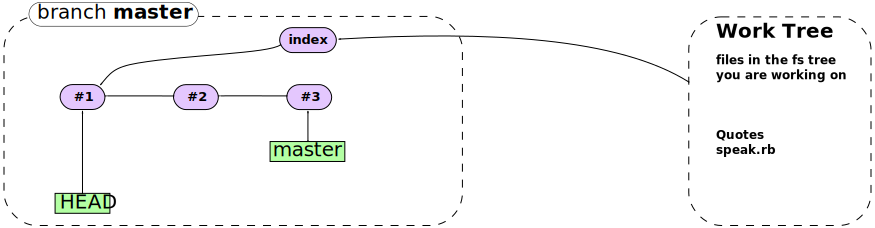
\includegraphics[scale=0.6]{../../../target/images/checkout-1.pdf}
        \caption{State or repository and work tree right after checking out the very fist commit.\label{fig:checkout-1}}
        \end{figure}
        \newpage
        \noindent We can go back to the last commit in our \texttt{master} branch by simply
        \begin{Verbatim}[frame=single]
 $ git checkout master
 Switched to branch 'master'
        \end{Verbatim}

        \noindent Then everything will look exactly like in Figure 5.

        Besides finding SHA1 values corresponding to specific commits there is another way to identify them (commits).
        If \texttt{HEAD} points to the last commit in the branch, then \texttt{HEAD\textasciitilde}
        or \texttt{HEAD\textasciitilde1} refers to previous commit and \texttt{HEAD\textasciitilde2} to the one before
        that. Thus we could have checked out the very first commit by simply
        doing "\texttt{git checkout HEAD\textasciitilde2}".

        To summarize. When checking out a specific commit, we move \texttt{HEAD} to that commit and make index and work
        tree exactly as that commit.

        If you do not specify commit and checkout one or more files, for example "\texttt{git checkout Quotes}" you
        will be reseting content of \texttt{Quotes} to what is in the index, NOT in checked out commit! You will be
        doing this operation quite often as you realize that you made some change in file in your work tree, but you do
        not need it and would like to discard local changes.

        \begin{Verbatim}[frame=single]
 $ echo "FOO" >> Quotes
 $ git status
 On branch master
 Changes not staged for commit:
   (use "git add <file>..." to update what will be committed)
   (use "git checkout -- <file>..." to discard changes in working directory)

        modified:   Quotes

 no changes added to commit (use "git add" and/or "git commit -a")
 $ git checkout Quotes
 $ git status
 On branch master
 nothing to commit, working directory clean
        \end{Verbatim}
        You can see that local modifications in \texttt{Quotes} are now gone. If however you stage changes for future
        commit by using "\texttt{git add}" you will need to use "\texttt{git reset}" to undo all of that. We will see
        how it works later.

        If you checkout past revision of some specific file things will look a bit differently. Git will keep HEAD
        wherever it point at now, synchronize content of just that file with checked out revision and add it to index.

        \begin{Verbatim}[frame=single]
 $ git checkout HEAD~2 Quotes
 $ git status
 On branch master
 Changes to be committed:
   (use "git reset HEAD <file>..." to unstage)

        modified:   Quotes
        \end{Verbatim}

        \begin{figure}[h]
        \centering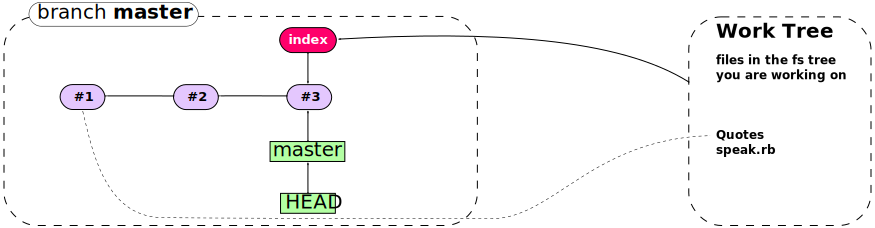
\includegraphics[scale=0.6]{../../../target/images/checkout-readme.pdf}
        \caption{After "\texttt{git checkout HEAD\textasciitilde2 Quotes}". The index and worke tree contain
          file \texttt{Quotes} as it is found in the commit \#1.\label{fig:checkout-readme}}
        \end{figure}

        \noindent If we are to commit now then content of \texttt{Quotes} we be reverted, but history of how we got
        here will be preserved.
        \begin{Verbatim}[frame=single]
 $ git commit -m 'Quotes reverted to its initial state'
 [master 67b2bd0] Quotes reverted to its initial state
  1 file changed, 3 deletions(-)
    \end{Verbatim}
    Indeed we can see that

        \begin{Verbatim}[frame=single]
 $ cat Quotes
 Beware of computer programmers that carry screwdrivers.
        \end{Verbatim}
        And state of our repository and work tree looks like this

        \begin{figure}[h]
        \centering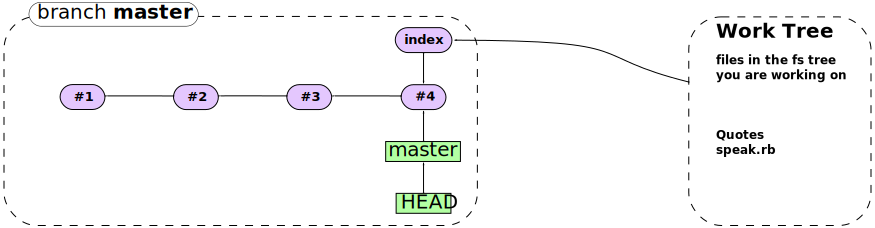
\includegraphics[scale=0.6]{../../../target/images/four-commits-wrong.pdf}
        \caption{State our repository and work tree after 4th commit. Content of \texttt{Quotes} file is reverted to
          how it was in commit \#1.\label{fig:4th-wrong-commit}}
        \end{figure}

        \section{Git Reset --mixed and --hard}

        Now we realize that we made a mistake and would like to undo it. We do not want actually file \texttt{Quotes} to
        be the same as in commit \#1. To undo that we will now modify history. This is a real danger zone.
        While "\texttt{git checkout}" allows us to move around history it does now allow us to screw it up, not so
        with "\texttt{git reset}". But actual difference between these commands is quite small.
        Command \text{git checkout} moves \texttt{HEAD} and a work tree a state recored in a particular commit, but
        leaves branch reference in place (in our case \texttt{master}). Command "\texttt{git reset}" moves branch head
        reference to the target commit and by proxy HEAD to the same state, since as you remember HEAD contains name of
        the branch head (aka. branch). And depending on the options used it will do different things to \texttt{index}
        and the work tree. Default reset strategy\footnote{Git actually has 5 different reset strategies. We discuss
          here only \texttt{soft}, \texttt{soft} and \texttt{mixed} and leave out \texttt{merge} and \texttt{keep}.}
        is known as {\em mixed}, which is that git will set index to the same commit that branch head points to, but
        will leave content of the work tree intact. This strategy can be evoked explicitly by use of "\texttt{--mixed}"
        option.

        \begin{Verbatim}[frame=single]
 $ git reset HEAD~
 Unstaged changes after reset:
 M      Quotes
        \end{Verbatim}
        \newpage
        \begin{Verbatim}[frame=single]
 $ git status
 On branch master
 Changes not staged for commit:
   (use "git add <file>..." to update what will be committed)
   (use "git checkout -- <file>..." to discard changes in working directory)

        modified:   Quotes

 no changes added to commit (use "git add" and/or "git commit -a")
        \end{Verbatim}
        And state of our repository looks like so

        \begin{figure}[h]
        \centering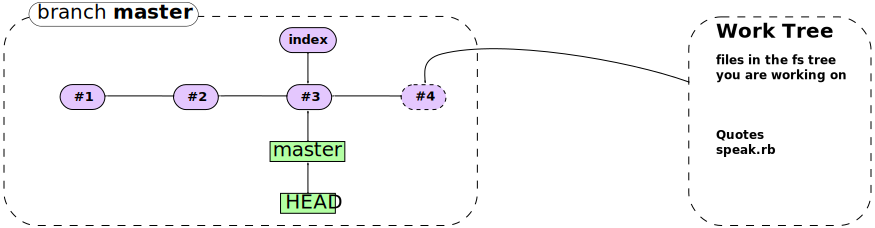
\includegraphics[scale=0.6]{../../../target/images/after-reset-1.pdf}
        \caption{State our repository and work tree after "\texttt{git reset HEAD\textasciitilde}". Content of index is
          the same as commit \#3, but content of the work tree is the same as commit \#4.\label{fig:after-reset-one}}
        \end{figure}

        The head of the branch \texttt{master} now points to commit before we screw up, i.e.
        commit \#3. \texttt{HEAD} points at \texttt{master} and index is the same as commit \#3 and state of the work
        tree is left in the state as it was at commit \#4. Notice that commit \#4 is still sitting somewhere inside of
        \texttt{.git/}, it is not lost, just does not have a simple symbolic reference to it\footnote{It actually does
        have reference even after extensive history manipulation. References to otherwise nameless commits are
        maintained in something called reflog. Also previous value of \texttt{HEAD} is always stored
        in \texttt{ORIG\_HEAD}}.

        More likely in this situation we want to make our work tree also look like in commit \#3 (new head of
        the \texttt{master} branch). To accomplish that we can use \texttt{reset} with \texttt{--hard} option. This
        will set work tree to the same state as index. Coincidentally that means that in the current
        state "\texttt{git reset --hard HEAD}" will have the same effect as "\texttt{git checkout README}".

        \begin{Verbatim}[frame=single]
 $ git reset --hard HEAD
 HEAD is now at bfafe95 New quote and hallo.rb
 $ git status
 On branch master
 nothing to commit, working directory clean
        \end{Verbatim}

        \begin{figure}[h]
        \centering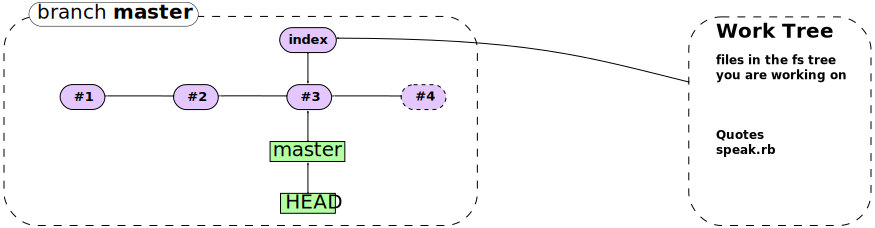
\includegraphics[scale=0.6]{../../../target/images/after-reset-hard.pdf}
        \caption{State our repository and work tree after "\texttt{git reset --hard HEAD\textasciitilde}".\label{fig:after-reset-hard}}
        \end{figure}

        \noindent Note again that commit \#4 is not lost and will still be around for some time until git will decide
        to clean it up even if we proceed making new commits. In the subsequent pictures we will remove this dangling
        commit and if commit \#4 will re-appear it will refer to completely new commit.

        \section{Checkout Revisited}

        Now that we really know about relationship between branches, index and work tree we can understand better
        what "\texttt{git checkout}" does. Lets add some more of the sage wisdom to file \texttt{Quotes}.
        \begin{Verbatim}[frame=single]
 $ echo "To err is human, but for a real disaster you need a computer." >> Quotes
 $ git add Quotes
        \end{Verbatim}
        Now our situation is exactly as in Figure \ref{fig:history-tree-index-committed}. If we fiddle
        with \texttt{Quotes} a bit more (add attribution as shown below) we will and up in the following state.
        \begin{Verbatim}[frame=single]
 $ echo "    - Anonymous" >> Quotes
        \end{Verbatim}

        \begin{figure}[h]
        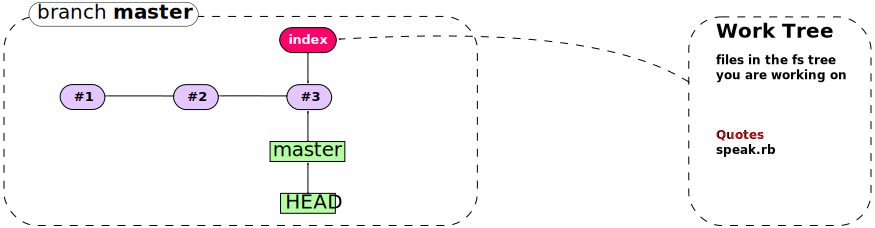
\includegraphics[scale=0.6]{../../../target/images/two-adds.pdf}
        \caption{Checked out commit, which is commit \#3, index and work tree are all different from each other.\label{fig:two-adds}}
        \end{figure}

        \noindent The index is different from the head and work tree is different from the index. If we now run "\texttt{git status}" we will see what we already seen before

        \begin{Verbatim}[frame=single]
 $ git status
 On branch master
 Changes to be committed:
   (use "git reset HEAD <file>..." to unstage)

        modified:   Quotes

 Changes not staged for commit:
   (use "git add <file>..." to update what will be committed)
   (use "git checkout -- <file>..." to discard changes in working directory)

        modified:   Quotes
        \end{Verbatim}
        But in view of preceding chapters comments on undoing these changes can now be easily understood. Command
        "\texttt{git checkout Quote}" will synchronize content of the \texttt{index} with the working tree. This will
        remove line "\texttt{- Anonymous}". And "\texttt{git reset HEAD}" will synchronize \texttt{index} with checked
        out commit essentially un-staging files from it. This operation would normally also move \texttt{HEAD}, but
        since target of the reset is \texttt{HEAD} itself that means that \texttt{HEAD} is left as it is. If you want
        to fully discard local changes as they differ from last commit, i.e. \texttt{HEAD}, then you can
        use "\texttt{git reset --hard}".

        \section{Branches Branching Out}
        So far our commits represent simple linear history. Of course in reality on any sufficiently large project
        history is never linear\footnote{In my experience in the main repository it is very much desirable to have
        history as linear as possible since any long lived branch presents two problems, one of merging it back to
        \texttt{master} and two it has tendency of farther branching complicating merge even more. But in your own local
        repository you will be creating and using many branches.}. Understanding branching is essential if we are
        not to be lost in the this forest of branches. First lets commit previous state.
        \begin{Verbatim}[frame=single]
 $ git add Quotes
 $ git commit -m 'Added disaster quote'
[master 855ccd5] Added disaster quote
 1 file changed, 2 insertions(+)
        \end{Verbatim}
        We now have simple linear history of just four commits. Remember that file \texttt{speak.rb} was introduced in
        the third commit. Lets imagine that that commit was used to release production software and now users enjoy the
        great functionality of the \texttt{speak.rb} program and development continued unabated in the \texttt{master}
        branch. Now it turned out that \texttt{speak.rb} contains a bug. A shocking development I know, but it turned
        out that our users actually wanted to see the sage wisdom accumulated in our \texttt{Quotes} file. Without
        affecting outgoing development we decide to fix that in a separate branch. To do that we checkout our commit
        where release happened, which is previous commit in our case and there create new branch \texttt{bugfix}.
        \begin{Verbatim}[frame=single]
 $ git checkout HEAD~
 $ git branch bugfix
 $ git checkout bugfix
        \end{Verbatim}
        This could actually be done using just one command "\texttt{git checkout -b bugfix HEAD\textasciitilde}", but I
        am showing it here in three steps to illustrate actual workings of this operation.
        After "\texttt{git checkout HEAD\textasciitilde}" our repository looks like this

        \begin{figure}[h]
        \centering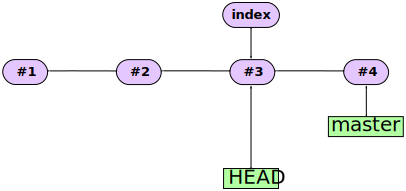
\includegraphics[scale=0.6]{../../../target/images/checkout-head-1.pdf}
        \caption{\label{fig:checkout-head-1}}
        \end{figure}

        \noindent Running "\texttt{git branch bugfix}" introduces new branch label.

        \begin{figure}[h]
        \centering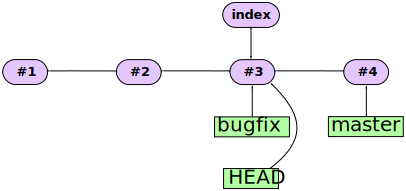
\includegraphics[scale=0.6]{../../../target/images/branch-bugfix.pdf}
        \caption{\label{fig:branch-bugfix}}
        \end{figure}

        \noindent Notice that \texttt{HEAD} is still detached. Adding commits at this point will still introduce
        dangling commits since \texttt{bugfix} label will not move. Branch label will move with new commits only
        if \texttt{HEAD} points at that branch label and not commit. Doing "\texttt{git checkout bugfix}" will do
        exactly that.

        \begin{figure}[h]
        \centering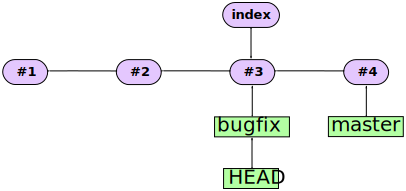
\includegraphics[scale=0.6]{../../../target/images/checkout-bugfix.pdf}
        \caption{\label{fig:checkout-bugfix}}
        \end{figure}

        \noindent You can see that creating a new branch is nothing more that creating branch label on any specific
        commit within the history. This is extremely light weight operation and exactly the reason why it is said that
        in git creating branches is cheap.

        Now we are ready to develop on our newly created branch \texttt{bugfix}. Lets fix the bug in
        the \texttt{hallo.rb} file and make a new commit.
        \newpage
        \begin{Verbatim}[frame=single]
 $ sed -i 's/puts.*$/puts File.open("Quotes", "r").read/' speak.rb
 $ git add speak.rb
 $ git commit -m 'speak.rb fixed'
 [bugfix cf97b8d] speak.rb fixed
  1 file changed, 1 insertion(+), 1 deletion(-)
        \end{Verbatim}
        And at this point our repository looks like this.

        \begin{figure}[h]
        \centering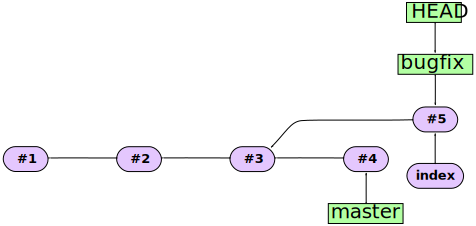
\includegraphics[scale=0.6]{../../../target/images/hallo-fixed.pdf}
        \caption{\label{fig:hallo-fixed}}
        \end{figure}

        \noindent We can now switch back and forth between branches by doing "\texttt{git checkout \$branch-name}"
        and the \texttt{HEAD}, the \texttt{index} and your work tree will follow. You can identify which branch you
        are on by doing

        \begin{Verbatim}[frame=single]
 $ git branch
 * bugfix
   master
        \end{Verbatim}

        \noindent This shows you all local branches\footnote{Concept of remote branches will be introduced later.
        Sufficient to say for now that they are related to ability of git to efficiently share its history with
        other git repositories.} and current branch is indicated by an asterisk.

        Separate development can now continue on both of these branches, but at some point you may want to merge one
        branch into another. Let say that we want to merge branches \texttt{bugfix} and \texttt{master} right now. We
        probably want to merge \texttt{bugfix} into \texttt{master} and not vice versa. To do that first we need to
        switch to \texttt{master} branch and then do merge.
        \begin{Verbatim}[frame=single]
 $ git checkout master
 $ git merge bugfix -m 'bugfix merge'
 Merge made by the 'recursive' strategy.
  hallo.rb | 2 +-
  1 file changed, 1 insertion(+), 1 deletion(-)
        \end{Verbatim}
        Git successfully replayed all changes made on the \texttt{bugfix} branch and applied them in the newly created
        merge commit. Things would not go so smooth if conflicting changes where made to the same file on both branches,
        but will get to that use case later. Our repository looks like this.

        \begin{figure}[h]
        \centering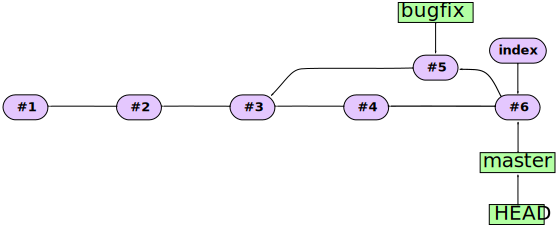
\includegraphics[scale=0.6]{../../../target/images/bugfix-merged.pdf}
        \caption{\label{fig:bugfix-merged}}
        \end{figure}
        \noindent Commit \#6 is in somewhat unique situation. It has two parents \footnote{We should note that commit
        numbers that you can see on the figures are completely irrelevant to actual commits, which are identified only
        by their SHA1 values. We however for the purpose of referring to commits in this text will often talk simply
        about commit number.}. Indeed if we look into this commit we will see following
        \begin{Verbatim}[frame=single]
 $ git cat-file -p $(cat .git/refs/heads/master)
 tree f15c536ac7a6c193446ceba193c478d079702de0
 parent 855ccd573362278e83463a08755d293794e911ed
 parent cf97b8d46a506b4a2065cb6c089a46f9e8e2c890
 author Mr. Smarty Pants <smarty.pants@shmoogle.com> 1463267185 -0700
 committer Mr. Smarty Pants <smarty.pants@shmoogle.com> 1463267185 -0700

 bugfix merge
        \end{Verbatim}
        The first parent refers to commit \#4, i.e. previous commit on the branch that we merged into, and second one
        refers to commit that was merged into current branch, i.e. commit \#5. We can identify first
        parent (primary one) simply as \texttt{HEAD\textasciitilde}. That is commit \#4. But how to reach 
        commit \#5? Turned out that there is another way to identify parent commits. \texttt{HEAD\^} is the same
        as \texttt{HEAD\textasciitilde} and \texttt{HEAD\^}\texttt{2} refers to commit that was merged into the current
        one, i.e. commit \#5 in our case.

        What git did here is it replayed all changes accumulated in \texttt{bugfix} branch and applied them
        in \texttt{master} creating new commit \#6, aka {\em merge commit}. It also formed link the branch that it was
        replaying. This link is important because development may continue on the \texttt{bugfix} branch and if we are
        to merge again in the future git will need to know where it merged before so as not to reply changes that were
        already merged.

        Git merge is a very powerful operation that can do many things. It can help you to untangle very complicated
        merges. While full description of all options applicable to "\texttt{git merge}" operation is outside of the
        scope of this booklet we will revisit it later when we learn about conflicts during merge and how to resolve
        them, and when we learn about remote tracking branches.

        \section{Reset --soft and revert}
        Lets say that upon some thinking we decided that in \texttt{master} branch we actually like how our code looked
        like at commit \#4 and we would like to restore it to that commit, but we do not want to loose our history by
        rewriting it. Therefore we want to create new commit that would be exactly like commit \#4. We can do that using
        following sequence of git commands.
        \begin{Verbatim}[frame=single]
 $ git reset --hard HEAD~
 $ git reset --soft ORIG_HEAD
 $ git commit -m 'Reverted to "Added disaster quote"'
 [master 37ce18e] Reverted to "Added disaster quote"
  1 file changed, 1 insertion(+), 1 deletion(-)
        \end{Verbatim}
        What actually happened here is following. After "\texttt{git reset --hard HEAD\textasciitilde}" our repository
        looks like so.
        \begin{figure}[h]
        \centering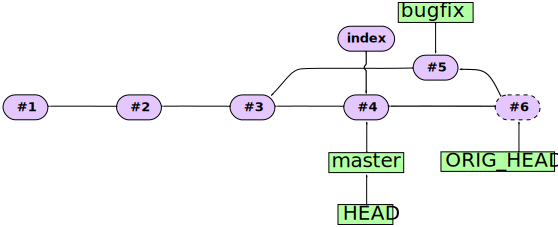
\includegraphics[scale=0.6]{../../../target/images/bugfix-merged-reset-hard.pdf}
        \caption{\label{fig:bugfix-merged-reset-hard}}
        \end{figure}

        \noindent Notice label \texttt{ORIG\_HEAD}. We already mentioned it several times, but here we are using it. What it
        is, is a label that points to the commit to which \texttt{HEAD} label was pointing to directly or indirectly
        before the last move. And it is also a file \texttt{.git/ORIG\_HEAD} just like \texttt{HEAD}.
        Since \texttt{HEAD} moved with the \texttt{master} branch label from commit \#6 to \#4
        label \texttt{ORIG\_HEAD} now points at the commit \#6. Hard reset synchronizes both the index and work tree
        with the target commit, but \texttt{--soft} one is different.
        After "\texttt{git reset --soft ORIG\_HEAD}" our repository looks like so.
        \newpage
        \begin{figure}[h]
        \centering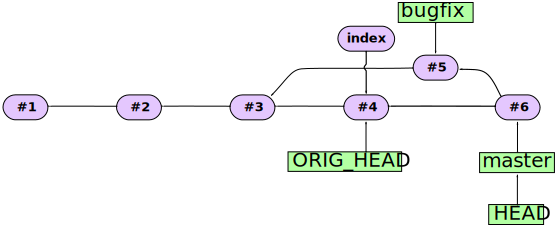
\includegraphics[scale=0.6]{../../../target/images/bugfix-merged-reset-soft.pdf}
        \caption{\label{fig:bugfix-merged-reset-soft}}
        \end{figure}

        \noindent Soft reset moves \texttt{HEAD} and the branch label, but leaves index and the work tree intact. Out
        index and work tree right now are exactly as they were at commit \#4. Performing commit right now will create
        new commit that looks exactly as commit \#4.
        \begin{figure}[h]
        \centering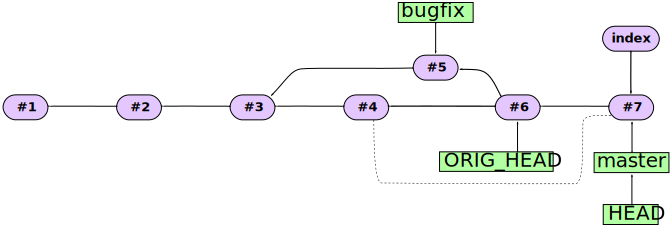
\includegraphics[scale=0.6]{../../../target/images/bugfix-merged-commit-revert.pdf}
        \caption{\label{fig:bugfix-merged-commit-revert}}
        \end{figure}

        \noindent This essentially undo merge commit \#6. The very same effect can be attained by
        using "\texttt{git revert}" command, which in the simplest form takes target commit pointer and creates new
        commit that reverts application of the target commit. And it can also take range of commits to create commit
        that reverses all commits in that range.

        We can now summarize actions of \texttt{checkout} and \texttt{reset} commands based on the what they do to
        the \texttt{HEAD}, branch label (\texttt{master} in our case), \texttt{index} and the work tree, i.e. which
        one of these for objects are modified upon which command.
        \newline
        \begin{center}
        \begin{tabular}{l | c | c | c | c}
            & \texttt{HEAD} & \texttt{master} & \texttt{index} & work tree \\
            \hline
            \texttt{git checkout} & \checkmark & & & \checkmark \\
            \hline
            \texttt{git reset --soft} & \checkmark & \checkmark & & \\
            \hline
            \texttt{git reset --mixed} & \checkmark & \checkmark & \checkmark & \\
            \hline
            \texttt{git reset --hard} & \checkmark & \checkmark & \checkmark & \checkmark \\
            \hline
        \end{tabular}
        \end{center}

        \section{Rebase}
        There is another way of merging two branches that often is preferable to what "\texttt{git merge}" does and
        that is {\em rebasing}. Lets do a little dance here with our current history. We need to do that to better
        illustrate benefits of rebasing. First lets add another commit in the \texttt{bugfix} branch.

        \begin{Verbatim}[frame=single]
 $ git checkout bugfix
 Switched to branch 'bugfix'
 $ echo 'puts "== The End =="' >> speak.rb
 $ git add speak.rb
 $ git commit -m 'Added end line printout'
 [bugfix a28f60c] Added end line printout
  1 file changed, 1 insertion(+)
        \end{Verbatim}
        And switch back to \texttt{master}.
        \begin{Verbatim}[frame=single]
 $ git checkout master
 Switched to branch 'master'
        \end{Verbatim}
        Now state of our repository looks like this
        \newpage
        \begin{figure}[h]
        \centering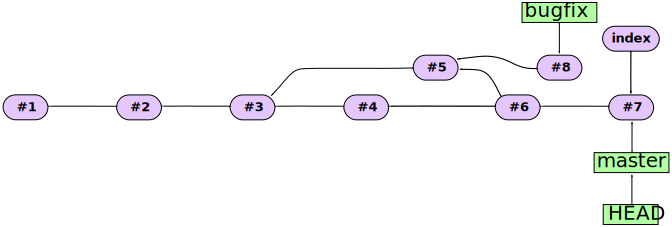
\includegraphics[scale=0.6]{../../../target/images/bugfix-second-commit.pdf}
        \caption{\label{fig:bugfix-second-commit}}
        \end{figure}

        \noindent Thoroughly confused by what we see and realizing that we do not actually need commit \#7 and do need
        results of work on the \texttt{bugfix} branch in the main branch we decide to rearrange things a bit. We also
        realize at this point that we will no longer have any more work done on the \texttt{bugfix} branch and will
        want to get rid of it, the branch that is.  Therefore first we do hard reset of \texttt{master} branch to
        commit \#4.
        \begin{Verbatim}[frame=single]
 $ git reset --hard HEAD~2
 HEAD is now at 855ccd5 Added disaster quote
        \end{Verbatim}

        \begin{figure}[h]
        \centering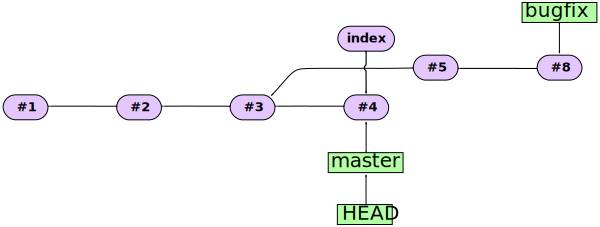
\includegraphics[scale=0.6]{../../../target/images/master-hard-reset-2.pdf}
        \caption{\label{fig:master-hard-reset-2}}
        \end{figure}

        \noindent If we are to merge \texttt{bugfix} into \texttt{master} we will introduce new commit that combines all
        the changes in all commits in \texttt{bugfix}. Looking at the code introduced in such merge commit it might
        actually be difficult to understand where and why certain code was introduced or removed. What if we could
        instead attach commit \#5 to the head of \texttt{master} branch. Command "\texttt{git rebase}" does exactly,
        except it does not just reattach \#5 to \#4, but takes all commits in the other (source) branch and replays them
        on top of the target branch, resolving conflicts while applying each commit one by one. First lets checkout
        the source branch that we will be rebasing.
        \begin{Verbatim}[frame=single]
 $ git checkout bugfix
 Switched to branch 'bugfix'
    \end{Verbatim}
    And then do rebase
        \begin{Verbatim}[frame=single]
 $ git rebase master
 First, rewinding head to replay your work on top of it...
 Applying: speak.rb fixed
 Applying: Added end line printout
        \end{Verbatim}
        This comment is actually quite illuminating. First git sets \texttt{HEAD} to the commit common to both
        branches, which is commit \#3. Then computed diff between \#3 and \#5 and then created new commit on top
        of \#4. This is expressed by {\em Applying ...} text. Then it applied second commit. If conflicts are discovered
        when applying commits then git will stop and will allow you to resolve them and then resume rebasing. It will do
        that until it will come to the head of the current branch and then change branch reference and
        the \texttt{HEAD}. And now out repository looks like this
        \newpage
        \begin{figure}[h]
        \centering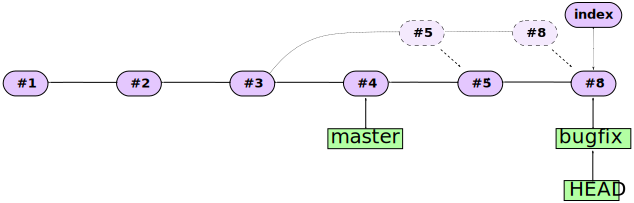
\includegraphics[scale=0.6]{../../../target/images/bugfix-rebased.pdf}
        \caption{After "\texttt{git rebase master}"\label{fig:bugfix-rebased}}
        \end{figure}

        \noindent Commits \#5 and \#8 are now gone and transformed into \#$5^{'}$ and \#$8^{'}$. They are different
        because they correspond to different states of the work tree from their original states since they incorporate
        commit \#4.

        But wait we are not done yet. Remember that we wanted \texttt{master} to be at the end of this chain of commits
        and branch \texttt{bugfix} gone. The first thing we can accomplish by the following commands.
        \begin{Verbatim}[frame=single]
 $ git checkout master
 Switched to branch 'master'
 $ git reset --hard bugfix
 HEAD is now at f5cbd2e Added end line printout
        \end{Verbatim}
        Now both \texttt{master} and \texttt{bugfix} point at the same commit \#$8^{'}$. And to delete reference
        label \texttt{bugfix} we do
        \begin{Verbatim}[frame=single]
 $ git branch -d bugfix
 Deleted branch bugfix (was f5cbd2e).
        \end{Verbatim}
        And now our repository looks very clean and simple but at the cost of potentially significant alterations of
        history.

        \begin{figure}[h]
        \centering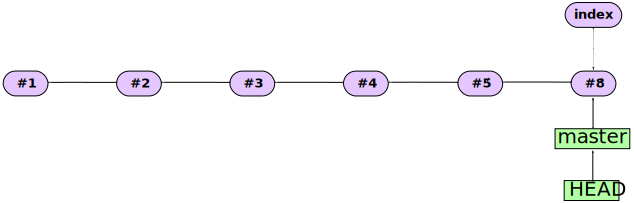
\includegraphics[scale=0.6]{../../../target/images/master-local-ff.pdf}
        \caption{\label{fig:master-local-ff}}
        \end{figure}

        \noindent Rebase can also be used to perform some deep alterations of history. This is not something you want to
        do very often, but when need arises you better know how to do that.

        Lets look at out current history.
        \begin{Verbatim}[frame=single]
 $ git log  --graph --oneline --pretty=oneline --decorate --all
 * f5cbd2e (HEAD, master) Added end line printout
 * e309c40 speak.rb fixed
 * 855ccd5 Added disaster quote
 * 3ab9407 New quote and speak.rb
 * 3f4a476 Added attribution.
 * cf82886 Initial commit.
        \end{Verbatim}
        In commit \#4 which is identified by SHA1 value 855ccd5... we added new text to the file \texttt{Quote}. This
        commit can be accessed by \texttt{HEAD\textasciitilde2} or \texttt{master\textasciitilde2}
        reference\footnote{Notice that you can use "\textasciitilde\$number" to identify parents at certain depth with
          any symbolic reference, be that \texttt{HEAD} or branch reference such as \texttt{master} or even commit
          SHA1 itself.}
        And we can therefore easily see what was done in that commit using "\texttt{git diff}"
        command\footnote{We can use "\texttt{git show master\textasciitilde2}" which will show commit object and all
          diffs introduced in that commit.}.
        \newpage
        \begin{Verbatim}[frame=single]
 $ git diff master~3 master~2
 diff --git a/Quotes b/Quotes
 index a78fe2a..d2d22bd 100644
 --- a/Quotes
 +++ b/Quotes
 @@ -2,3 +2,5 @@ Beware of computer programmers that carry screwdrivers.
      - Leonard Brandwein
  Never trust a computer you can’t throw out a window.
      - Steve Wozniak
 +To err is human, but for a real disaster you need a computer.
 +    - Anonymous
        \end{Verbatim}
        Let say that we decided to get rid of this commit and therefore change introduced by it. Not only we do not
        like this quote attributed to some Anonymous, but we want to erase any trace of it from our history. What
        that means is that we want commit \#$5^{'}$ to be connected to \#3 instead of \#4. Note that
        commit \#$5^{'}$ will actually stay intact and new commit \#$5^{''}$ will be introduced. In other words, we
        would like our history to look like this.

        \begin{figure}[h]
        \centering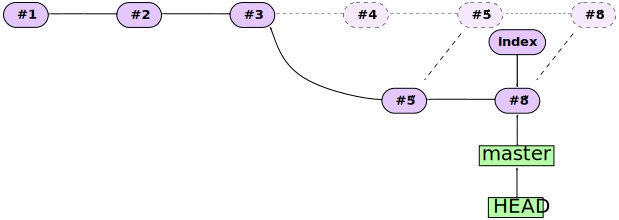
\includegraphics[scale=0.6]{../../../target/images/rebase-onto.pdf}
        \caption{Desired history manipulation that will effectively remove commit \#4. \label{fig:rebase-onto}}
        \end{figure}

        \noindent This will have the same effect as removing commit \#4 from the history. We can accomplish that using
        command "\texttt{git rebase --onto}". We will use three arguments for this command even though the last one
        can be omitted as it is implied.

        \section{Cherry Picking}
        \section{Remotes}
        \section{Refspec}
\end{document}
